% Scan Raggio Iniziale (E=61keV)
\begin{frame}
\frametitle{Scan Raggio Iniziale (E=61keV)}
\framesubtitle{Equilibrio "Finger Like"}
\begin{columns}
	\begin{column}{0.4\textwidth}
		\begin{center}
		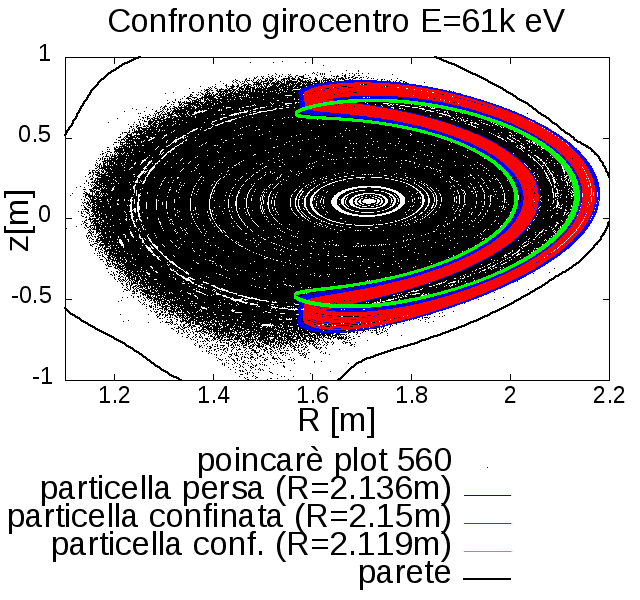
\includegraphics[scale=0.28]{Immagini/Simulazioni/Single/560/confronto.png}
		\end{center}
	\end{column}
	\begin{column}{0.4\textwidth}
		\begin{center}
		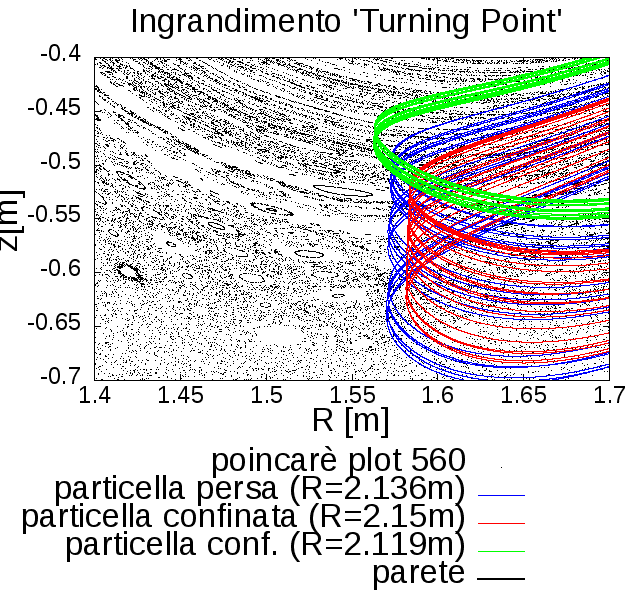
\includegraphics[scale=0.28]{Immagini/Simulazioni/Single/560/confronto_zoom.png}
		\end{center}
	\end{column}
\end{columns}
\end{frame}

% Scan Raggio Iniziale (E=61keV)
\begin{frame}
\frametitle{Scan Raggio Iniziale (E=61keV)}
\framesubtitle{Equilibrio Stocastico}
\begin{columns}
	\begin{column}{0.4\textwidth}
		\begin{center}
		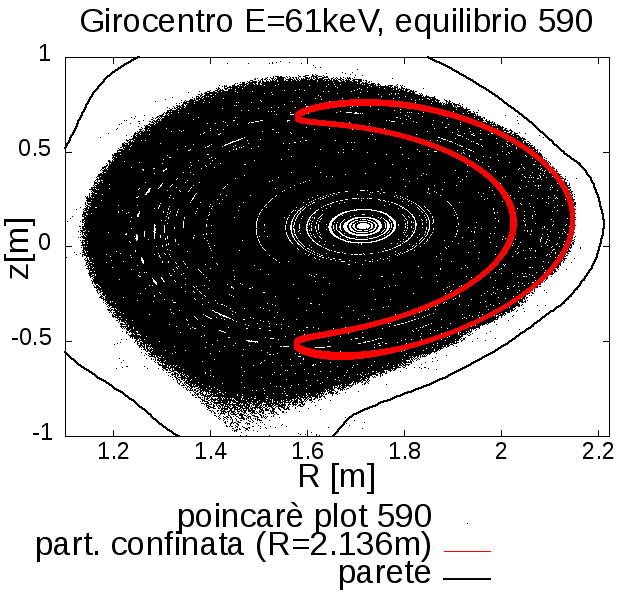
\includegraphics[scale=0.28]{Immagini/Simulazioni/Single/590/R_2136_E_61k.png}
		\end{center}
	\end{column}
	\begin{column}{0.4\textwidth}
		\begin{center}
		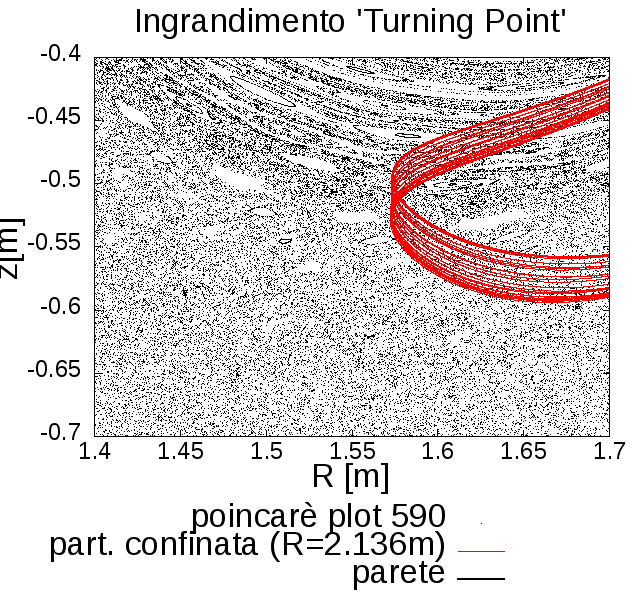
\includegraphics[scale=0.28]{Immagini/Simulazioni/Single/590/confronto_zoom.png}
		\end{center}
	\end{column}
\end{columns}
\end{frame}



% PERDITE 590
%\begin{frame}
%\frametitle{Scan Energia vs Raggio Iniziale}
%\framesubtitle{Equilibrio Stocastico}
%		\begin{center}
%		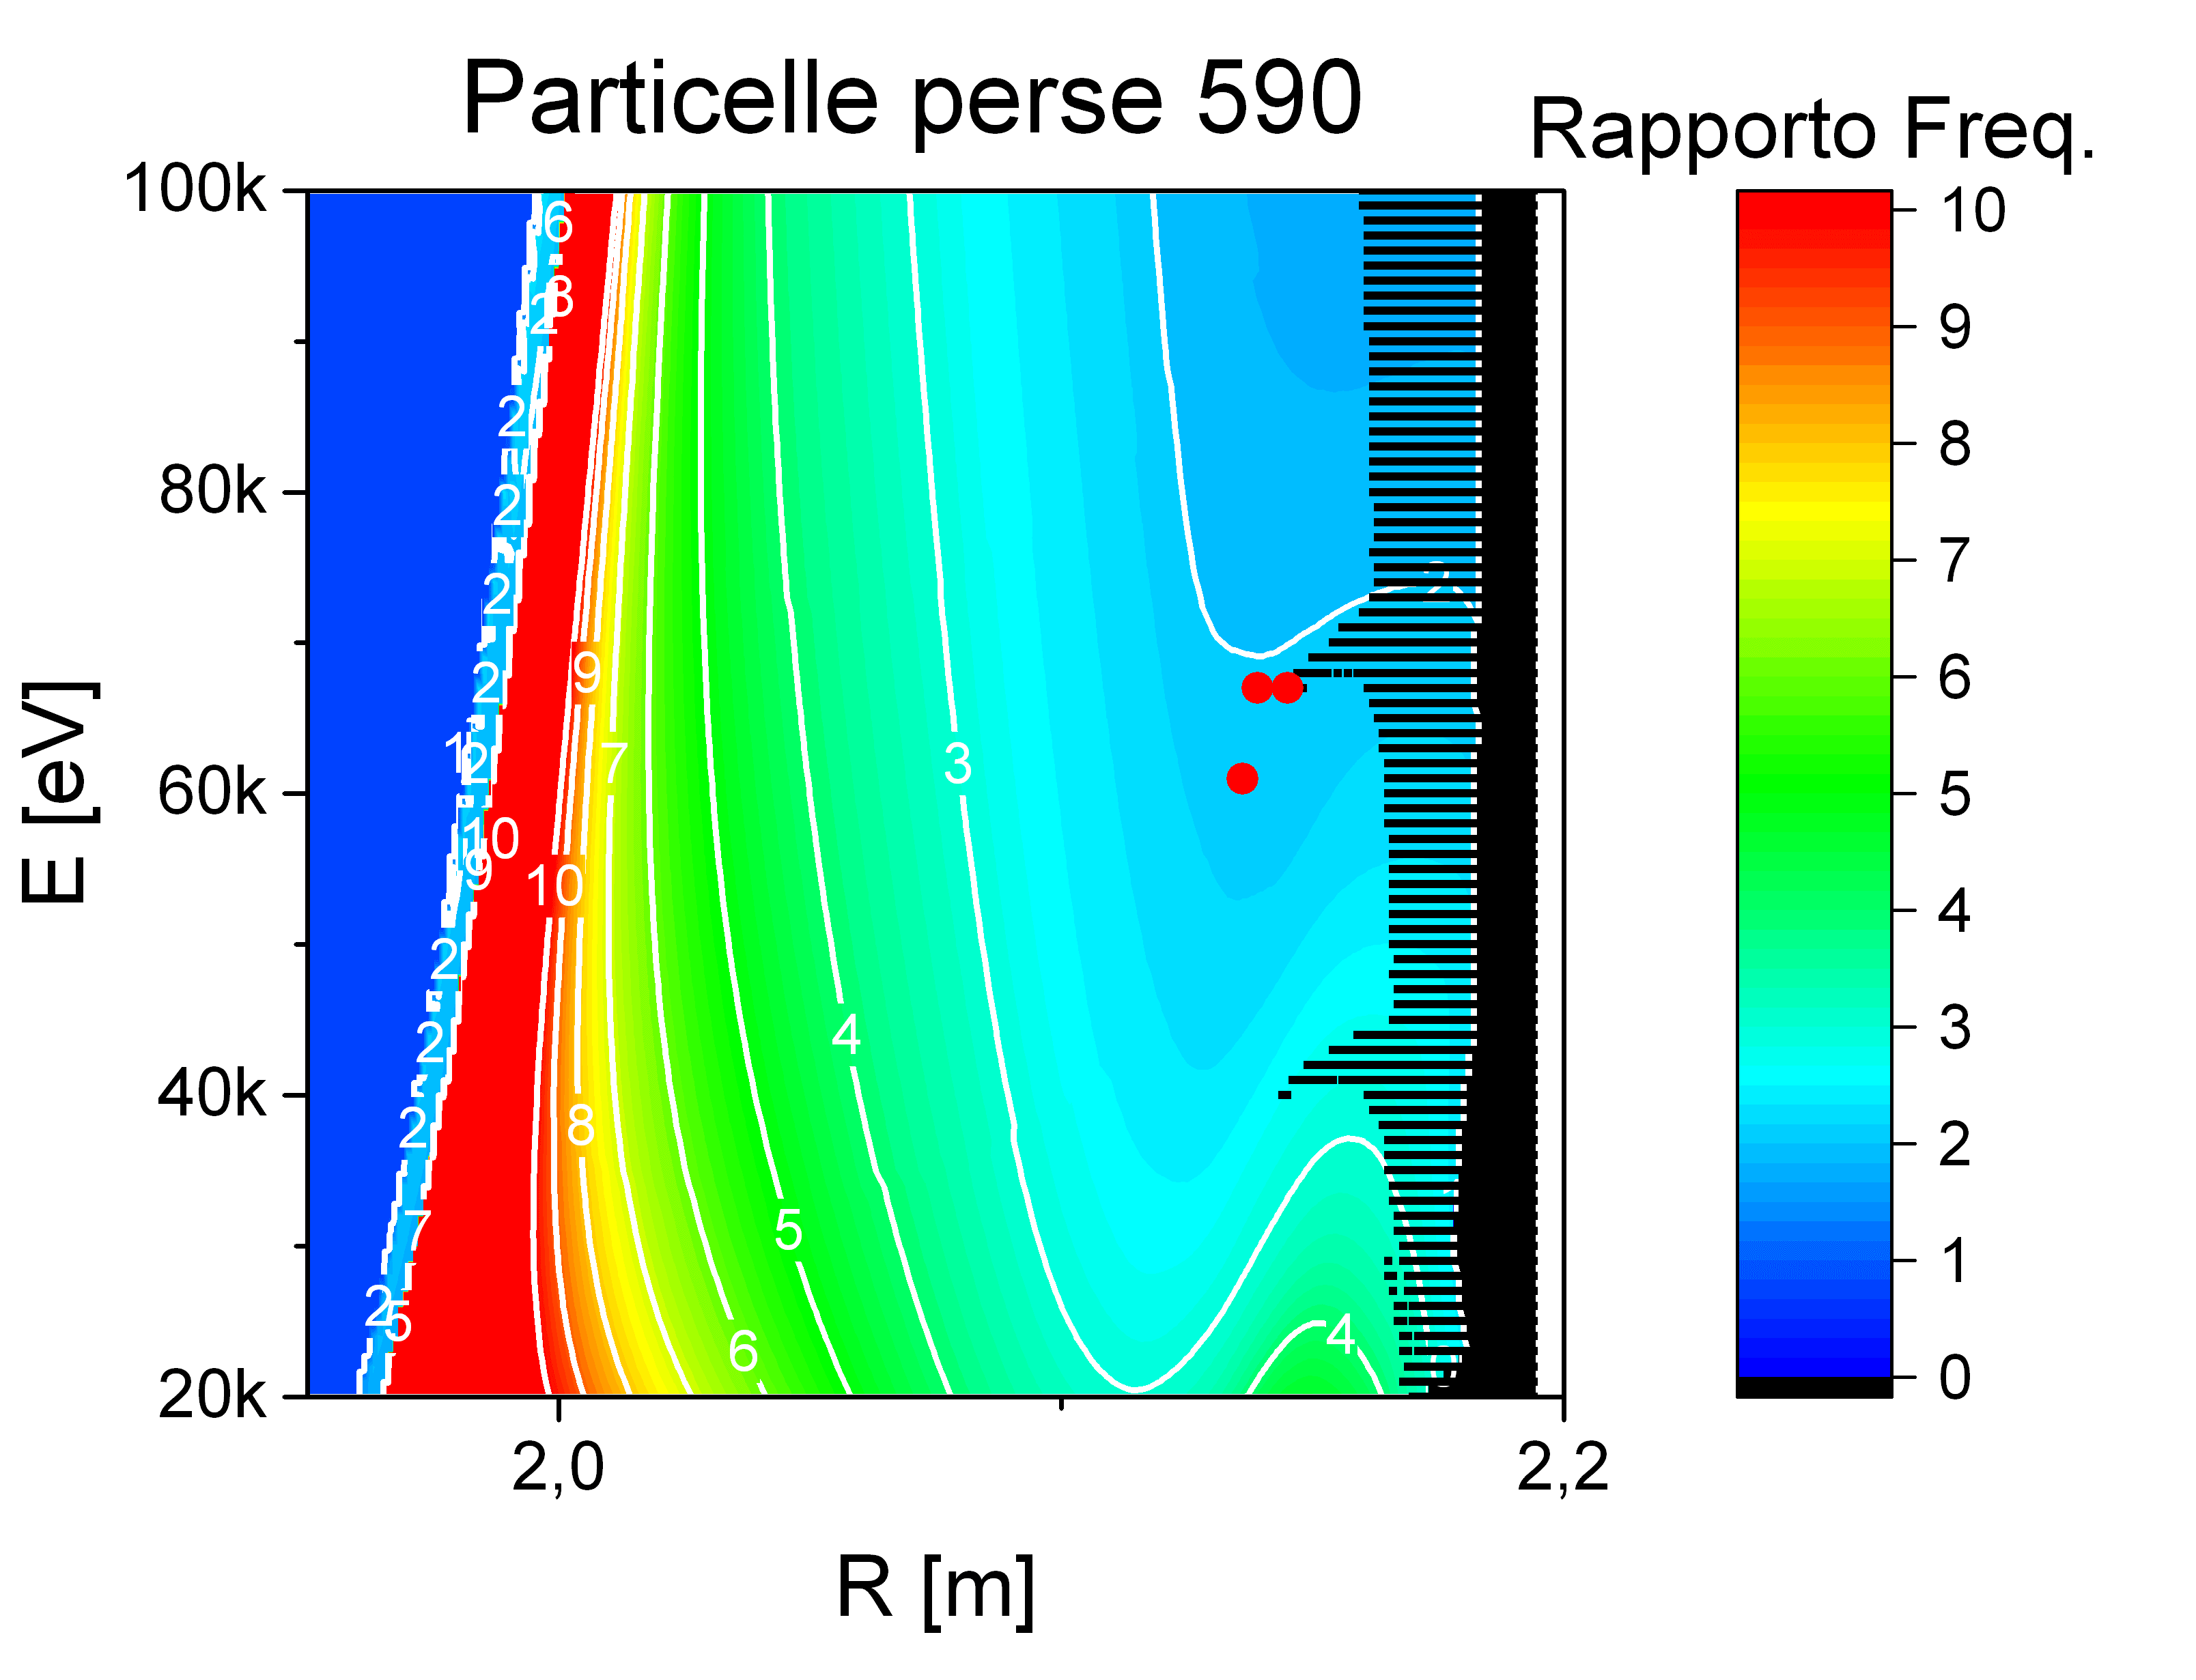
\includegraphics[scale=0.35]{Immagini/Simulazioni/Risonanze/particle_losses_590.png}
%		\end{center}
%\end{frame}

% Scan Raggio Iniziale (E=67keV)
\begin{frame}
\frametitle{Scan Raggio Iniziale (E=67keV)}
\framesubtitle{Equilibrio Stocastico}
\begin{columns}
	\begin{column}{0.4\textwidth}
		\begin{center}
		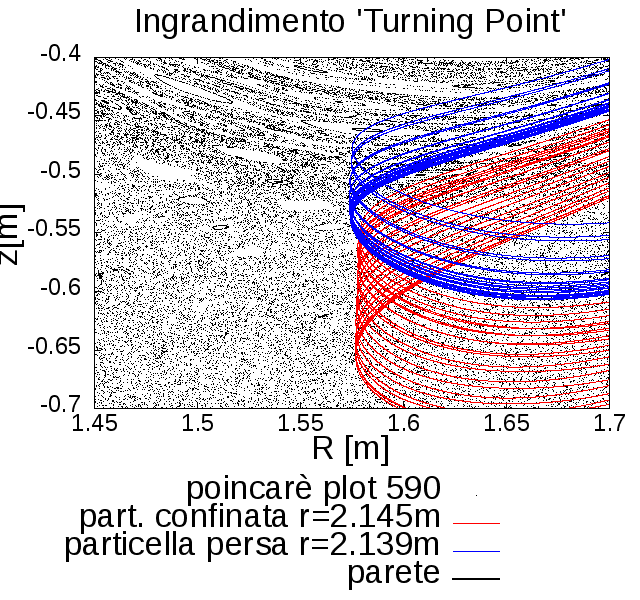
\includegraphics[scale=0.28]{Immagini/Simulazioni/Single/590/confronto_67.png}
		\end{center}
	\end{column}
	\begin{column}{0.4\textwidth}
		\begin{center}
		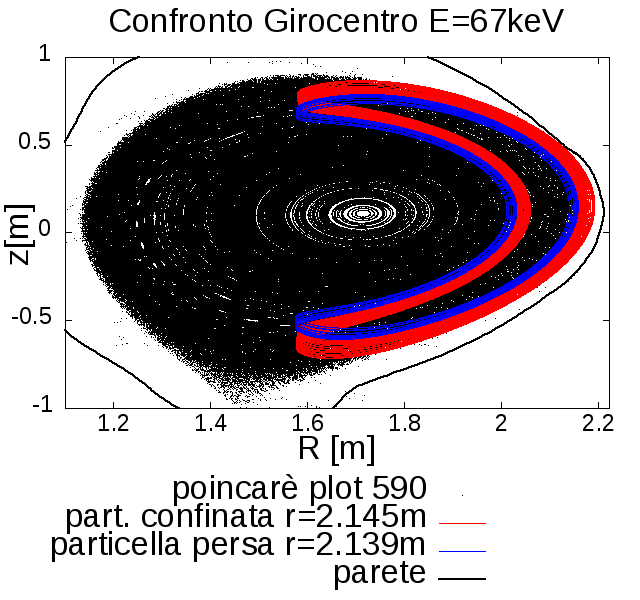
\includegraphics[scale=0.28]{Immagini/Simulazioni/Single/590/confronto_67_all.png}
		\end{center}
	\end{column}
\end{columns}
\end{frame}